\section{Introduction}

    Up until now, we have restricted the identification of excesses to within a 75~pc volume around the Sun. As discussed in the \textbf{which section} of Chapters~\ref{chap:iddisks} and \ref{chap:confirm}, this is because any stars with excesses identified within this volume have accurate parallaxes, and make excellent targets for additional disk characterization through high-contrast imaging techniques. In addition, the stars have very little to no line-of-sight extinction from interstellar dust. These are stars within a structure known as the Local Bubble \citep{Lallement2003}. 
    
    
    However, the nearby solar neighborhood has been heavily scrutinized for debris disks by the last thirty years of disk detections, by missions from \iras, \spitzer, and now \WS. If one considers the census of debris disks within 120~pc, roughly 80\%  reside within a volume 75~pc, with $\sim$20\% within the volume slice between 75 and 120~pc. However, by looking at the distribution of \hip\ main-sequence stars in 120~pc, the ratio of stars between 0--75~pc and 75--120~pc is nearly 50/50. Therefore, if we are to believe the constant incidence rate of disks derived by the last thirty years of disk detections, there are a vast number of new debris disks that have not yet been identified. 
    
    %lit known 75: 606
    %lit 75-120: 161
    %lit total: 767
    
    Since we already have the necessary tools in place, and our parent sample of stars (see section blah in chapter blah) already extends out to 120~pc, it may seem like a relatively simple matter to merge the science and parent samples and identify excesses of the entire parent sample. However, stars beyond 75~pc are more likely to be affected by line-of-sight extinction increases. The interstellar dust will decrease the intensity of shorter wavelength light from a star. If one is looking for IR excesses using short wavelength data, the line-of-sight extinction will artificially boost any measured excess mid-IR flux, thereby introducing an additional false-positive source. Thus, accurate assessment of an excess beyond 75~pc for a large sample of stars, similar to the ones we have been utilizing, requires a priori knowledge of the extinction level for all our stars at the various \WS\ bands.
    
    To largely remove the effects of interstellar extinction, one can use the $W3$ and $W4$ bands to search for $W3-W4$ single color excesses. Interstellar extinction is greater at the $W1$ and $W2$ bands than at $W3$. In addition, the data show a relatively flat slope for the IR extinction curve between 10 and 20\micron\ \citep{Wang2014}. Thus, any extinction felt by $W3$ will be roughly of the same magnitude felt by $W4$, preserving the measured infrared excess flux. Thus, in this study, we investigate the presence of warm and faint excesses at $W4$ all the way out to 120~pc, by identifying significant $W3-W4$ color excesses.
    
    
    \textbf{Write something about galactic plane stuff}


\section{Sample Selection}

    We derived our sample from the same set of \hip\ stars as was discussed in \S~2 of Chapter~\ref{chap:iddisks}. We selected main sequence \hip\ stars with well behaved \WS\ All-Sky photometry in the $W3$ and $W4$ bands. Our parent sample consists of stars within 120~pc with Tycho colors constrained to $-0.17~\rm{mag}< B_T-V_T< 1.4~\rm{mag}$ (late B to K spectral types). Since we are only interested in the $W3-W4$ colors for this study, saturation corrections to the $W1$ and $W2$ photometry was not necessary. Filters from \S~2.2.1 in Chapter~\ref{chap:iddisks}, that are relevant to the $W3$ and $W4$ bands, were placed on our parent sample of stars. 
    
    In contrast to the last two studies, we include stars within the galatic plane into our parent sample for this study. This adds an additional 766 \hip\ stars with well behaved $W3$ and $W4$ photometry to our parent sample, bringing the number of stars in our $W3-W4$ parent sample to 15199. We would also like to point out that in this study, we increase our science sample out to 120~pc. Therefore, our science and parent samples are equivalent.

   \subsection{Culling the Parent Sample via \textit{unWISE} Images}\label{sec:unwise_reject}
    
    The higher angular resolution \WS\ images from the \textit{unWISE} image service \citet{Lang2014} affords us the opportunity to identify sources that are potentially contaminated from blended point sources (e.g., active galactic nuclei, luminous infrared galaxies, other stars, etc.) or extended emission from interstellar IR nebulosity. Contaminated sources will manifest themselves as astrometric offsets, calculated from the centroid positions between the $W3$ and $W4$ images or by using different sized apertures in the $W4$ band to calculate the star's astrometric offset. In Chapter~\ref{chap:confirm}, our goal was to identify contaminants amongst the excesses we had already discovered. In contrast, here we aim to reject potentially contaminated stars \textit{prior} to excess identification.
    
    In short, we aimed to identify point source contamination by rejecting stars with significant $W3$ to $W4$ relative centroid offsets ($\Delta r_{W3,W4} = \left|\vec{r}_{_{W3}} - \vec{r}_{_{W4}}\right|$), as well as identify and reject stars contaminated from extend source emission from their measured $W4$ to wide-$W4$ centroid offsets ($\Delta r_{W4} = \left|\vec{r}_{_{W4}} - \vec{r}_{_{W4},_{wide}}\right|$). For this analysis, we extracted centroids for all the stars from their \textit{unWISE} $W3$ and $W4$ images. A detailed description of these procedures is discussed in \S~\ref{sec:unwise_rejectmethod}. 
    
    We looked for contaminated sources by identifying stars with the largest statistically significant offsets with respect to the distribution of offsets created from the parent sample of stars. The density clouds in Figures~\ref{fig:unwise_w3w4} and \ref{fig:unwise_w4w4} show the distributions of 15304 stars from our $W3-W4$ parent sample, prior to applying the filters we placed in \S~2 of Chapter~\ref{chap:iddisks}. The plots show the distribution of our stars' $W4$ SNRs as a function of the $W3$ to $W4$ relative centroid offsets ($\Delta r_{W3,W4}$) as well as a function of the $W4$ to wide-$W4$ centroid offsets ($\Delta r_{W4}$). Low $W4$ SNR stars will be affected more by small scale variations in the background, and hence the scatter of offsets at lower SNRs will shift toward higher separations, while the opposite effect will occur for stars at higher SNRs. Thus, a natural upper envelope to the distribution arises, and stars above that envelope will be rejected. 
    
    %=============================================================
    % unWISE W3/W4
    %=============================================================
    \begin{figure}
    \centering
    \includegraphics[width=\textwidth]{Ch5/w3w4_snrvsep_galplane}
    \caption[Rejected \textit{unWISE} stars using $W3$ to $W4$ offsets]{Distribution of relative positional offsets of stellar centroids between $W3$ and $W4$ using images from the \textit{unWISE} image service, plotted with respect to the $W4$ SNR calculated from the \textit{unWISE} images. The black/gray density cloud represents the density of 15304 Hipparcos stars from the parent 120~pc sample. The black-dotted line represents our separation cut-off ($1/3$~pixels) below which stars are not rejected. Our rejection threshold (orange dotted line) was fit to $\{\Delta r_{j,max}\}$ (dark-blue diamonds), calculated as described in Section~ \ref{sec:unwise_rejectmethod}. Rejected stars to the right of the vertical dotted black line and above the orange dotted line (red squares) are deemed to be contaminated by an unrelated nearby point or extended source seen in projection.}
    \label{fig:unwise_w3w4}
    \end{figure}
    %=============================================================


    %=============================================================
    % unWISE W4/W4
    %=============================================================
    \begin{figure}
    \centering
    \includegraphics[width=\textwidth]{Ch5/w4w4_snrvsep_galplane}
    \caption[Rejected \textit{unWISE} stars using $W4$ to $W4$ offsets]{Distribution of relative positional offsets of stellar centroids between a narrow 2.5~pixel radius and wide 10~pixel radius apertures, as described in Section~\ref{sec:centroid_calc}. The plot elements are the same as those described in Figure~\ref{fig:unwise_w3w4}. Rejected parent sample stars are marked as red circle.}
    \label{fig:unwise_w4w4}
    \end{figure}
    %=============================================================
    
    The upper envelopes in both distributions were calculated by fitting an exponential curve to the $\Delta r_{j,max}$ points in log-log space, and using the same techniques outlined in \S~\ref{sec:unwise_rejectmethod} to calculate $\Delta r_{j,max}$. We also kept the same fixed 1/3~pixel lower limit for both analyses. In other words, stars are not rejected below this separation. The red points in Figures~\ref{fig:unwise_w3w4} and \ref{fig:unwise_w4w4} show stars from the parent sample that are likely contaminated by blended point sources or extended emission. Two hundred and twenty stars were rejected from the $\Delta r_{W3,W4}$ vs. $W4$ SNR analysis, and 738 stars were rejected from the $\Delta r_{W4}$ vs. $W4$ SNR analysis. The union of these two sets show that a total of 919 stars should be rejected, though only 897 stars from our filtered parent sample match the astrometric outliers. Out of the 897 rejected stars, 174 reside in the galactic plane, leaving 592 galactic plane stars in our parent sample. Our final $W3-W4$ parent sample is comprised of 14302 main-sequence \hip\ stars with well behaved $W3$ and $W4$ photometry. 
    
    The 897 rejected stars account for 6.27\% of the original parent sample. Based on our assumptions, the photometry of all these stars must be contaminated by either extended emission or a blended point source. Though it is difficult to verify this claim, we show in the following section that the distribution excess significances are much better behaved after removing these stars, implying to some extent that our analysis is doing a good job of cleaning the parent sample of stars. 
    

\section{IR Excess Identification}

    Our excesses are selected using the same procedures described in \citet{Patel2014} and the improved methods for identifying single-color excesses in \S~\ref{sec:improved_detection}. We use Equation~\ref{eq:old_sig}, to determine the significance of the color excess for each star. Since we only wish to identify excesses with $W3-W4$ colors only, the excess significance takes on the form of
    
    \begin{equation}\label{eq:excess_sig_w3-w4}
    \Sigma_{E[W3-W4]} = \frac{W3-W4-W_{34}(B_T-V_T)}{\sigma_{34}},
    \end{equation}

    \noindent where $W_{34}(B_T-V_T)$ is the empirically derived $W3-W4$ photospheric colors, and $\sigma{34}$ is the total error term which includes the photometric and photospheric uncertainties. Both of these quantities are derived in \S~\textbf{XXX} in Chapter~\ref{chap:iddisks}. 
    
    Figure~\ref{fig:sige_w3-w4} shows the distribution of $\Sigma_{E[W3-W4]}$ for our parent sample of stars. We selected excesses such that their $\Sigma_{E[W3-W4]} \geq \Sigma_{E[W3-W4]_{99.5}}$. $\Sigma_{E[W3-W4]_{99.5}}$ is our 99.5\% confidence threshold, beyond which 0.5\% of stars are false-positive detections. In other words, our analysis is set to identify excesses up to a 99.5\% false-discovery rate (FDR). $\Sigma_{E[W3-W4]_{99.5}}$ was calculated using the same procedures that we describe in \S~\textbf{XXX}. For this analysis, we determined $\Sigma_{E[W3-W4]_{CL}}=2.894$, and is marked as the dotted black line n Figure~\ref{fig:sige_w3-w4}. 

    %=============================================================
    %  Color Distribution
    %=============================================================
    \begin{figure}
    \centering
    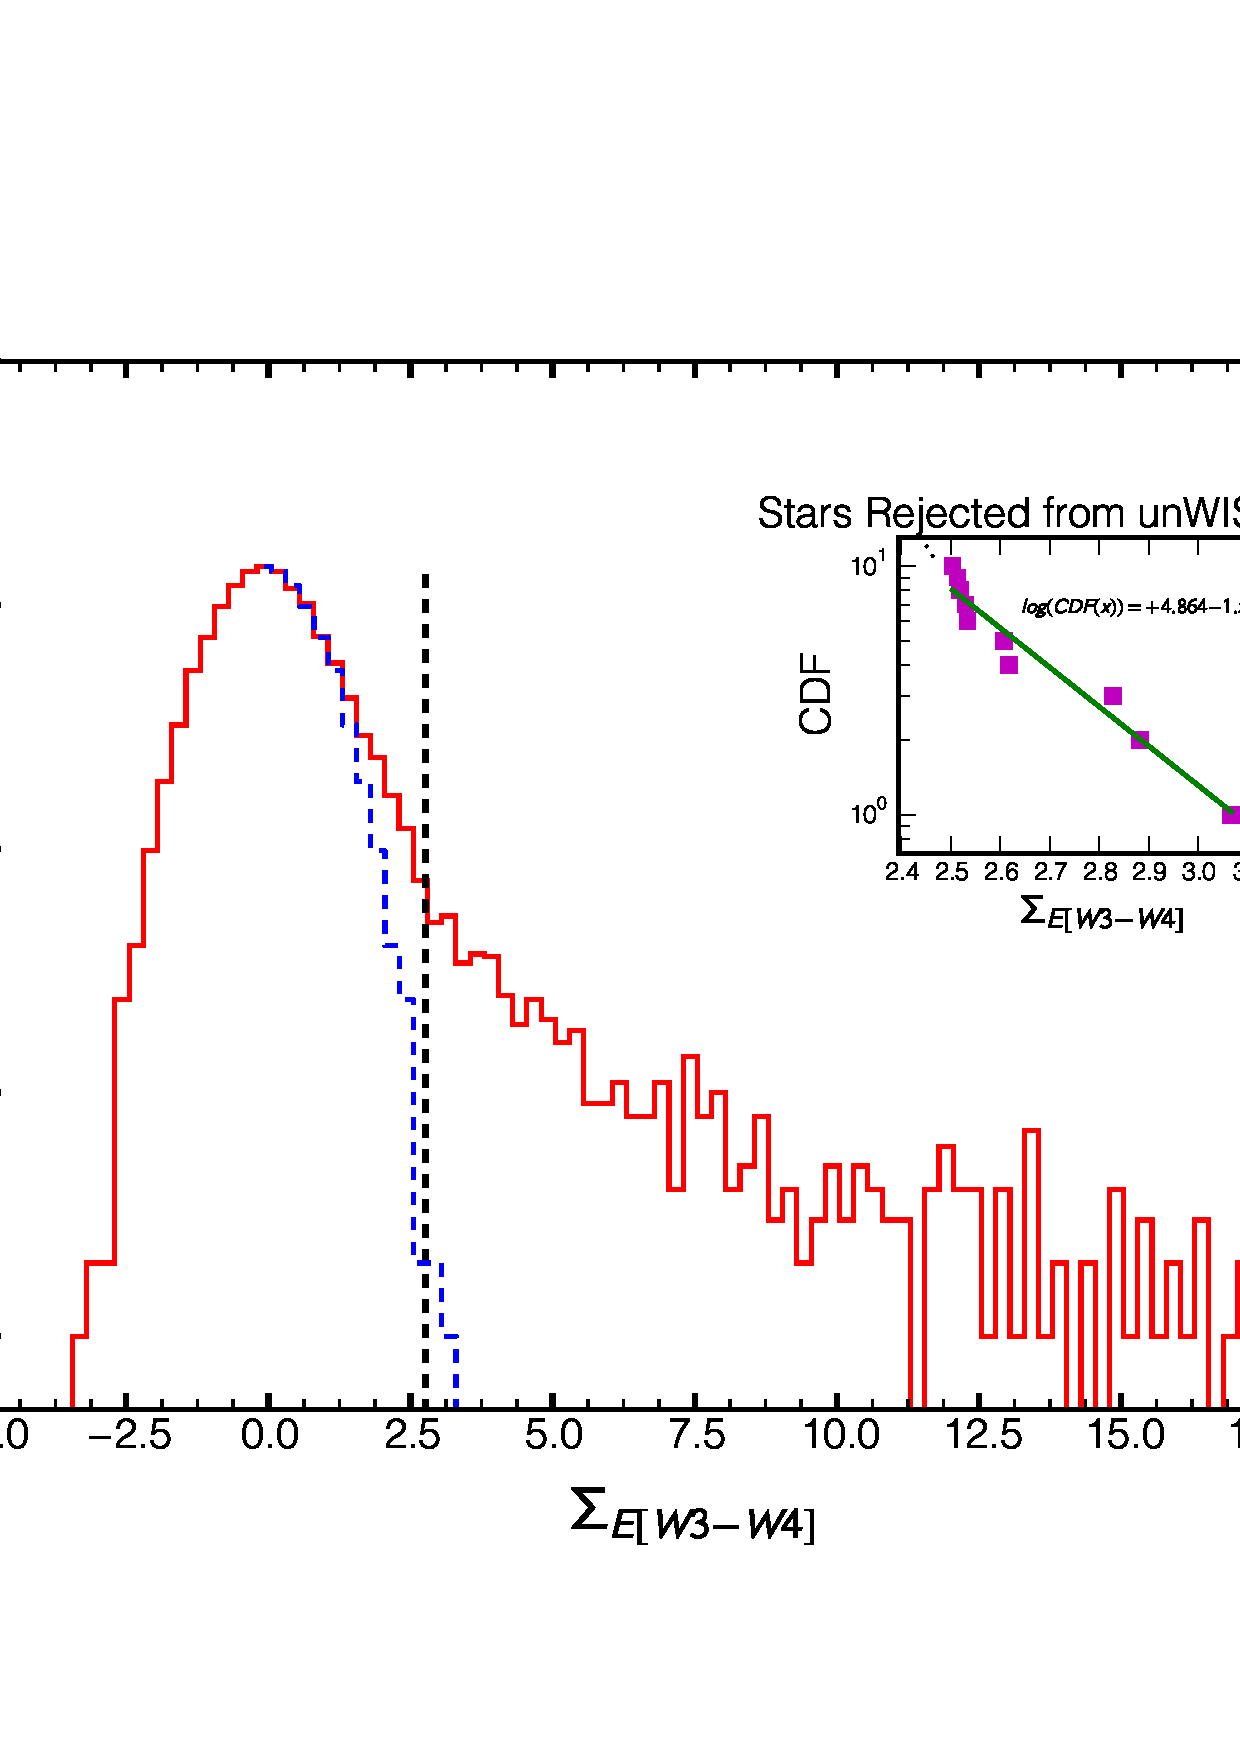
\includegraphics[width=\textwidth]{Ch5/W3-W4_colordist_removedunwisestars_galplane}
    \caption[Distribution of $\Sigma_{E[W3-W4]}$ in 120~pc]{}
    \label{fig:sige_w3-w4}
    \end{figure}
    %=============================================================

    Our selection process identified 640 stars with significant $W4$ excesses. Out of the 640, we expect 3.2 (=640$\times$0.5\%) of our excesses to be spurious false-positives. In addition, we still need to remove excesses which may be contaminated from interstellar cirrus clouds. Our astrometric offset rejection in \S~\ref{sec:unwise_reject} does not guarantee rejection of all such contaminated stars, as large patches of extended interstellar cirrus may appear as uniform back emission to our centroiding algorithm. Thus, we visually inspected the four band \WS\ Atlas images and removed 119 sources that appear to be contaminated from interstellar cirrus. Since we are using a subset of the parent sample from \citet{Patel2014}, contaminated excesses we rejected in that study appear in this one as well. Therefore, we list all the rejected sources in Table~\textbf{XXX}, except for those which we listed in previous studies. 
    
    In total, we identified 522 significant $W3-W4$ excesses out to 120~pc. Out of these, 210 were identified by our previous two studies in Chapter~\ref{chap:iddisks} and \textbf{xxx}. This leaves 312 stars for which we have not previously reported an excess from our past studies.
    
    \section{Results}
    
    From the 522 debris disks we identified in this study, 16 reside within the galactic plane $|b|<5^{\circ}$. \textbf{Need to write somethign else about this. Come back to it later}.
    
    Out of the 312 $W4$ excesses that we had not identified in our previous studies, 225 stars are new 22\micron\ excesses, previously unreported in the literature. Of these, 222 stars do not have previous detection of an excess at any wavelength in the literature. In addition, eight of our new excesses reside within 75~pc. Hence, we are also detecting new excesses within a volume which we had previously searched. 
    
    We also determined the stellar and dust properties of the 522 excess stars, which are listed in Table~\textbf{XXX} and \textbf{XXX}, respectively. We performed the same analysis as in \S~\textbf{XXX} in Chapter~\textbf{XXX} to derive these parameters by performing photospheric model fits. We used NextGen grid models from \citet{Hauschildt1999} to fit the optical and near-IR photometry from \hip\ and \mass. In a similar manner to that described in \S~\textbf{XXX}, we scaled the derived photospheric model to the mean of the $W1$, and $W2$ photometry. We used the $W4$ excess flux and $W3$ or 3$\sigma$ upper limit to the $W3$ excess flux to determine the best fit blackbody temperature for the dust emission. We have also placed upper limits to all of our dust temperature estimates using the 3$\sigma$ upper limit to the $W3$ excess flux. This allows us to constrain the dust properties to some extent, since we do not have longer wavelength information for all of our stars. Without this information it is difficult to ascertain whether the dust is emitting from warm grains, or whether the excess we measure is the Wien emission of much colder dust. 
    
   % Reuslts:
  %  - # of excesses
  %  - # of new 10--30\micron\ excesses
  %  - # of excesses within gal plane: 16/592 = 2.7\% pm 0.7
  % -- % of stars from parent sample in gal plane: 592/14302 = 4.1% pm 0.2
    %Stars outside galactic plane before unwise: 14433, cut = 2.904
    %stars incluidng galactic plane before unwise: 15199, cut =3.701
    %stars otuside gal plane after unwise: 13710, cut = 2.776
    %stars inside gal plan after unwise: 14302, cut = 2.894
    %-mention how much larger the threshold was if we didn't remove those contaminated stars
    
    %\subsection{Warning of Different Releases}
    %\textbf{Not sure if this should be moved to the discussion section}

\section{Discussion}

    \subsection{Survey Sensitivity}
    
    A goal of this study was to identify faint warm debris disks with \WS, though our detections need to be placed in context to literature excesses. We cannot characterize the full extent of the disk brightness $f_d$ (Equation~\ref{eq:fd}) since we only have excess flux information at $W3$ and $W4$. However, compare the relative flux at $W4$ ($R_{22}$; Equation~\ref{eq:rel_excess}) of the candidate debris disk hosts from our survey to the relative flux of disks detected at similar wavelengths. Although it would make sense to compare the relative flux of our disks at 22\micron\ to those detected by \iras\ at 25\micron, the latter sample is rather small given that the majority of \iras\ disks were detected in the far-IR. 
    
    Instead, we compare the relative flux at $W4$ for our excesses, to those excesses detected from the \spitzer at 24\micron\ using MIPS. \citet{Chen2014} conducted a study to characterize the excess SEDs of 571 stars with archival \textit{Spitzer}/IRS observations, supplemented with data from observations using \spitzer/MIPS at 24\micron. In addition, \citet{Lawler2009} conducted a survey to detected
    
    
    
     search for bona-fide excesses --- in large part due to the numerous filters we placed to cleanse our dataset of false-positives and  --- 

    importance to solar system.


    %=============================================================
    %  WISE Excess Sensitivity
    %=============================================================
    \begin{figure}
    \centering
    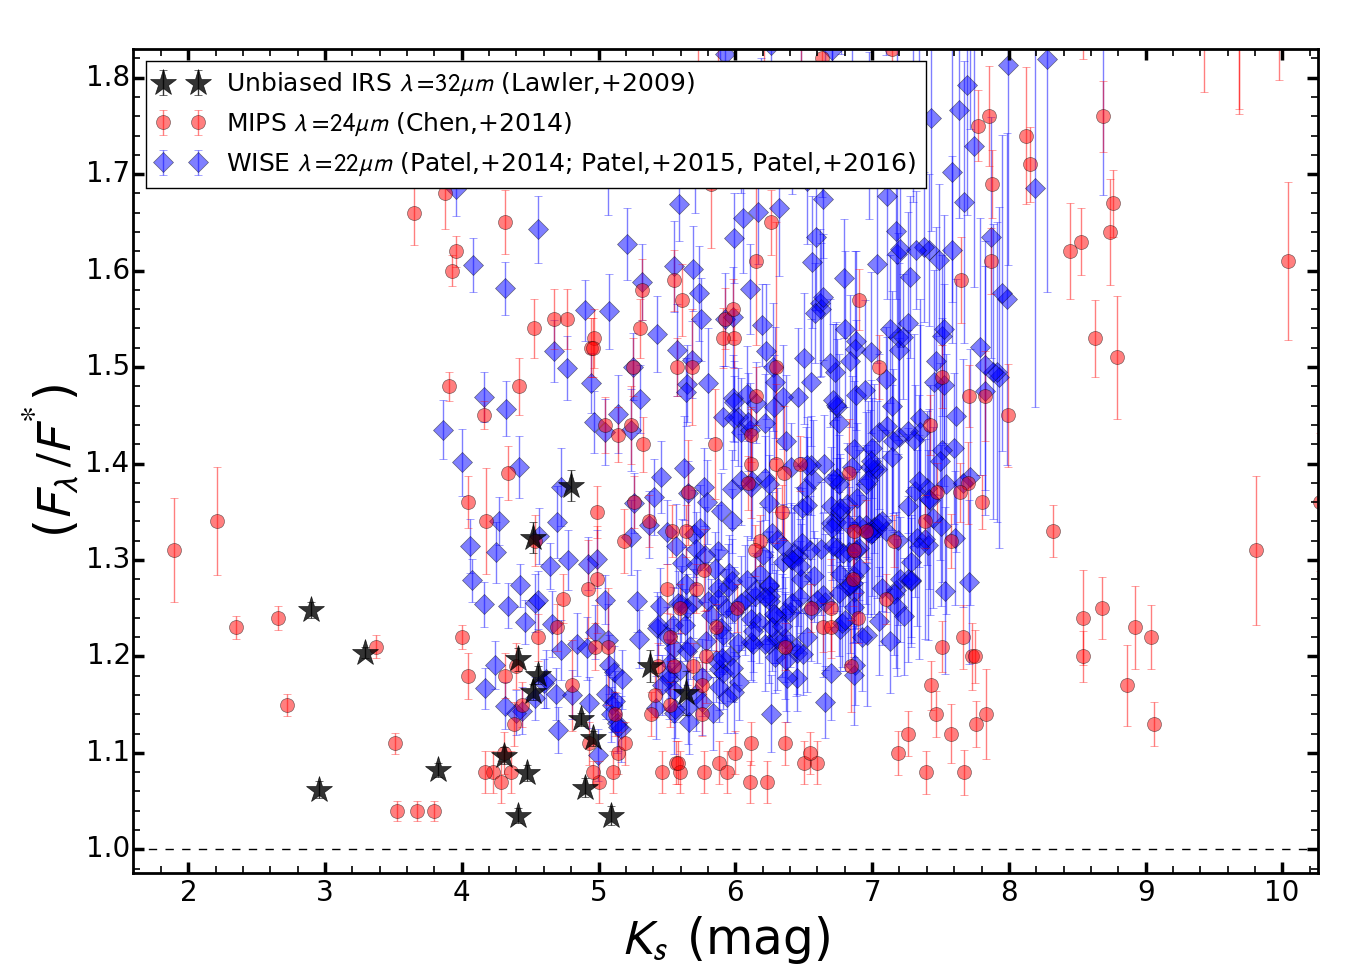
\includegraphics[width=\textwidth]{Ch5/relflux_wise_mips_irs_120pc}
    \caption[WISE Disk Sensitivity]{}
    \label{fig:wise_relflux}
    \end{figure}
    %=============================================================




    %=============================================================
    % My WISE vs. Their WISE
    %=============================================================
    \begin{figure}
    \centering
    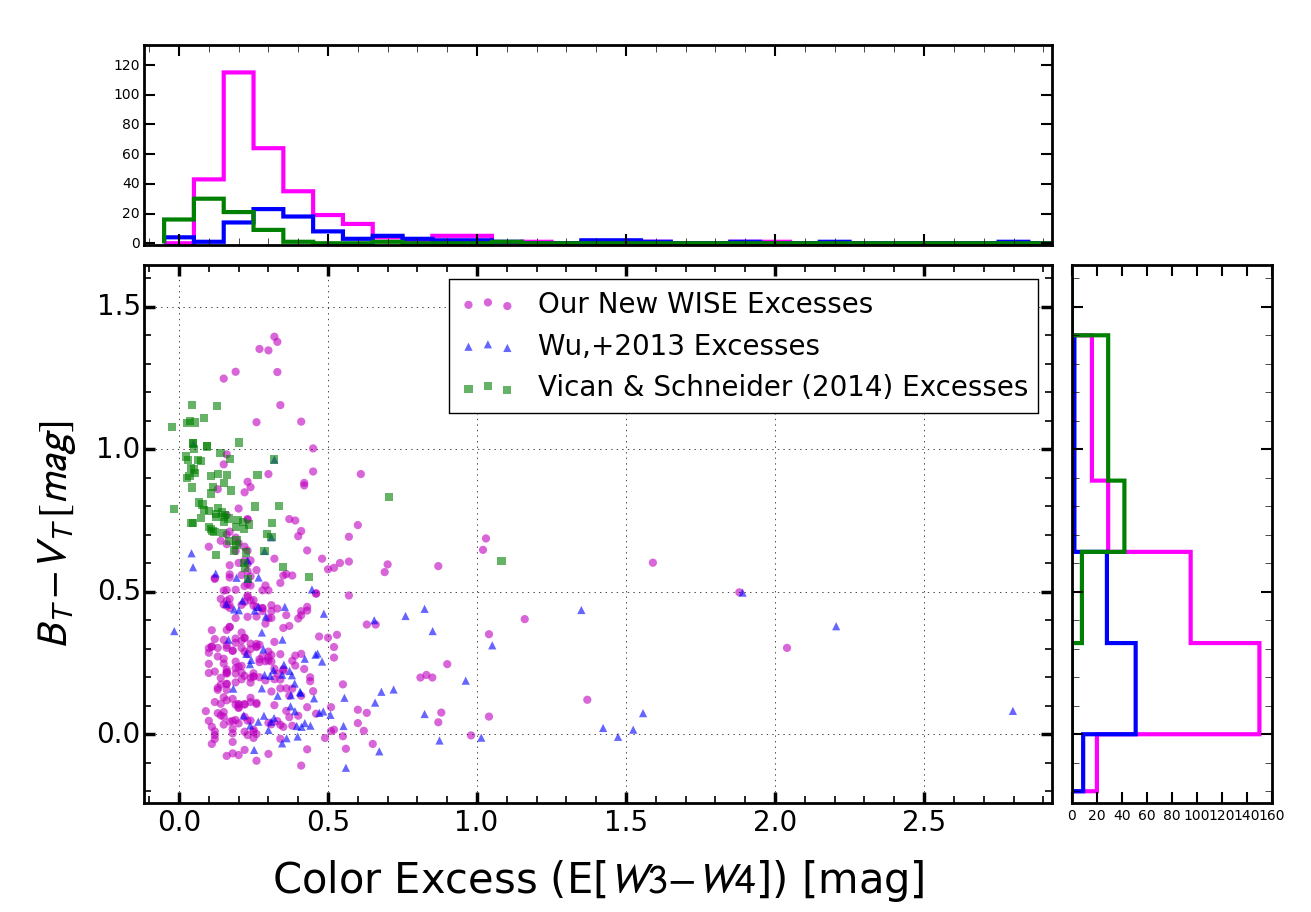
\includegraphics[width=\textwidth]{Ch5/wise_vs_wu_120pc}
    \caption[My WISE Disks vs. Other WISE Disks]{}
    \label{fig:wise_v_wise}
    \end{figure}
    %=============================================================
    
    
    

    
    
    \subsection{Overall Expansion of Disk Census}

    %=============================================================
    %  120 pc incidence rates
    %=============================================================
    \begin{figure}
    \centering
    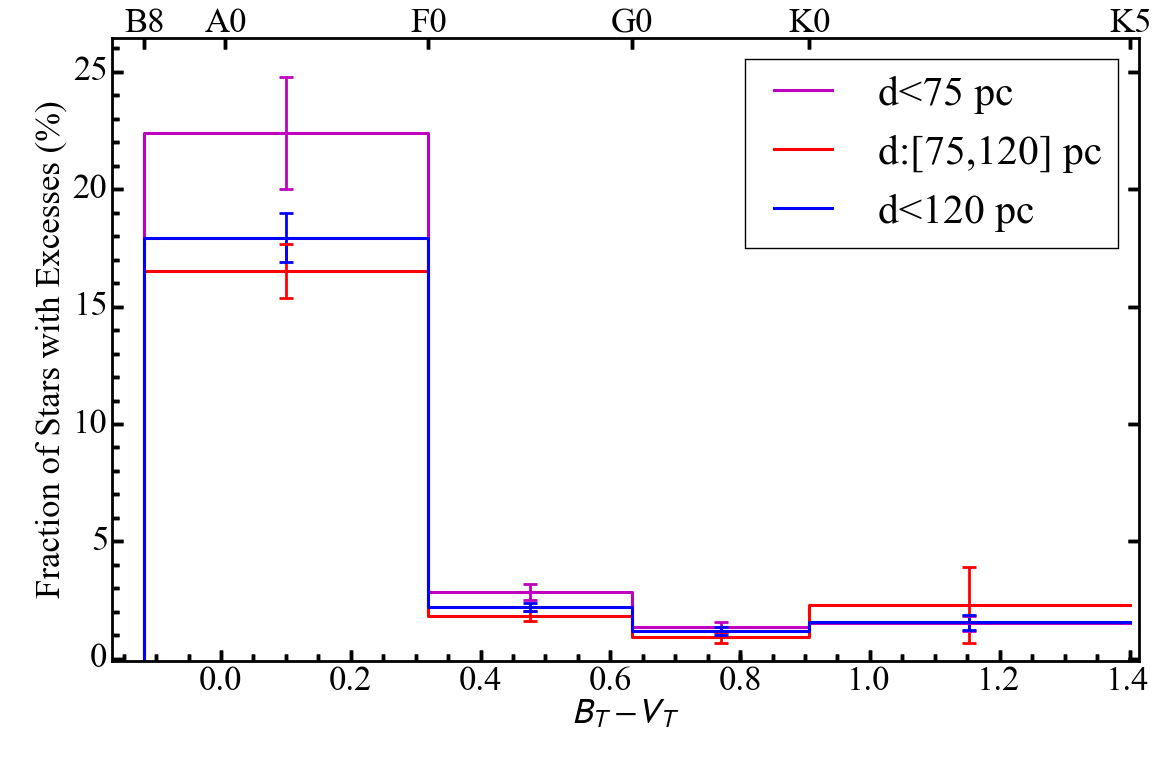
\includegraphics[width=\textwidth]{Ch5/incidencerates_120pc}
    \caption[Incidence of Excesses]{}
    \label{fig:incidence_rates}
    \end{figure}
    %=============================================================
    
    
    
    %=============================================================
    % WISE vs. Literature
    %=============================================================
    \begin{figure}
    \centering
    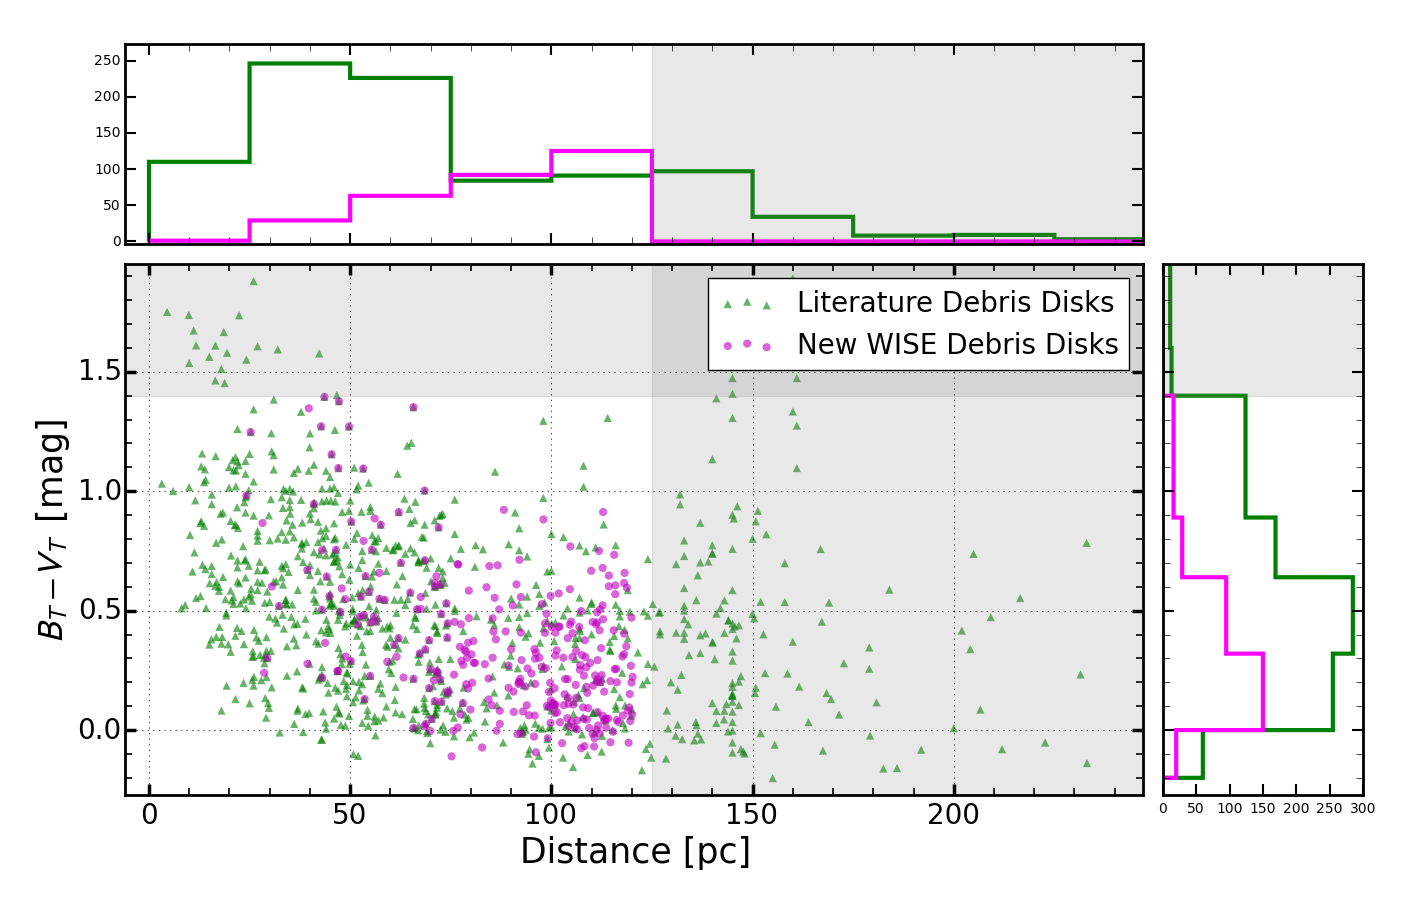
\includegraphics[width=\textwidth]{Ch5/wise_lit_120pc}
    \caption[Comparison of All Known Debris Disks To Those Detected by \WS]{}
    \label{fig:wise_v_lit}
    \end{figure}
    %=============================================================


    
    
    
   % - visually rejected stars -- more are removed than need be